% !TEX encoding = UTF-8 Unicode
% !TEX root = project.tex

\section{Evaluation}
\label{sec:finding}

In order to evaluate the effectiveness of our tool, we ran experiments on existing projects in GitHub. We only selected Java-based projects as we used Java specific tools to generate static call hierarchies. We wrote a script in Ruby\footnote{\url{https://www.ruby-lang.org/en/}} which could download the source code associated with pull requests\footnote{\url{https://help.github.com/articles/proposing-changes-to-a-project-with-pull-requests/}} using the Github API\footnote{\url{https://developer.github.com/v3/}}. The retrieved pull request information and the associated file information were saved into a set of database tables for further analysis. Then we further filtered the list down to make sure that only issue related pull request files were considered. This data was compared against the strongly connected components data obtained by running our implementation of the Kosaraju-Sharir algorithm, which was also used for populating the front-end user interface. This comparison would give us an idea of how helpful our tool would have been, in retrospect. 

\subsection{Evaluation Setup}

We gathered data from 4 projects in GitHub: Guava~\cite{guava}, Retrofit~\cite{retrofit}, Twitter4j~\cite{twitter4j} and Scribejava~\cite{scribejava}. The project descriptions are listed in Table \ref{tab:evaluationprojects}. The main programming language used in these projects is Java. From these small sample set of data that we evaluated against, our tool was able to successfully predict (recall) 36\%, 66\%, 5\% and 14\% respectively for the projects Guava, Twitter4j, Retrofit and Scribejava. 

\begin{table}[h]
\centering
\begin{tabular}{ll}
\hline
Project & Description \\
\hline
Guava & Google Core Libraries for Java \\
Retrofit & Type-safe HTTP client \\
Twitter4j & Java library for the Twitter API \\
Scribejava & Simple OAuth library for Java \\
\hline
\end{tabular}
\caption{Projects used for evaluation.}
\label{tab:evaluationprojects}
\end{table}

All of these open source GitHub projects had several pull requests and a lot of these pull requests were created for issues. One of the criterion that we used to select projects from Github is that they are not new projects which tend to have less number of pull requests and they may not be helpful for our experiments. Another criterion is to have a fair number of pull requests and a good mix of java files in them. Third criterion is that they can be packaged to form a jar file which our tool consumes. Although it was an option for us to implement the tool which could accept a project folder, it made more sense for us to package it as a jar file, which contained class files after building the project.

\subsection{Evaluation Results}

For the Guava project, we only took the core module which itself gave a good sized project to work on. We found 817 files using our tool that is part of the strongly connected components of the project and is predicted to be more defect-prone. But only 143 files were retrieved from the pull request of the corresponding module. When we matched these files, we found that 52 files were common between these two sets. That gave us a recall of 36\%, i.e., 52 out of 143 files. With respect to precision, only 52 out of 817 files were correct, i.e., only 6\% precision for the Guava project.

\begin{figure}[h!]
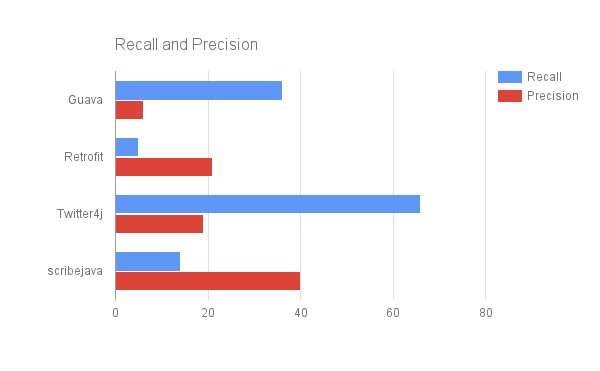
\includegraphics[width=8cm]{recall-precision}
\caption{Bar chart showing values of precision and recall}
\label{fig:precision_recall}
\end{figure}

The second project that we analysed was Retrofit. The tool predicted that 55 files were more defect-prone from the strongly connected components calculation. From the data we obtained from Github for this project, there were 214 files. Only 12 files were found to be common between these sets. That gave us a recall of 5\% (i.e., 12 out of 214 files) and a precision of 21\% (i.e., 12 out of 55 files).\\

The third project that we analysed was Twitter4j, in which we took only the core module which was big enough for our analysis. A total of 245 files were predicted to be defect-prone by the tool based on its strongly connected component calculation. 72 files were obtained from the Github repository for the project which were part of the pull requests. We found that there are 48 files which are common between these two sets. So the recall came out to be 66\% (48 out of 72 files) and precision calculated was 19\% (48 out of 245 files).\\

The last project that we analysed was Scribejava, and we took only the core module. This was comparatively a smaller project as compared to the other ones. A total of 25 files were predicted by the tool to be defect-prone based on the module's strongly connected components. 73 files were obtained from the Github repository for the project which were part of the pull requests. 10 files were found to be common between these two sets. That made the recall to be 14\% (10 out of 73 files) and the precision to be 40\% (10 out of 25).\\

Figure~\ref{fig:precision_recall} shows the graphical representation of the precision and recall obtained for projects that we took for analysis. Scribejava project has the highest value for Precision (40\%) and second lowest value for Recall (14\%).\\

There were no patterns that emerged from these figures, the reason for which we conjecture is because of the varied number of pull requests and the files associated with them. One project had a lot more files associated with them forming more number of strongly connected components. More experimental studies would be required to come out with a good explanation for these figures.\\

\begin{figure*}[h!]
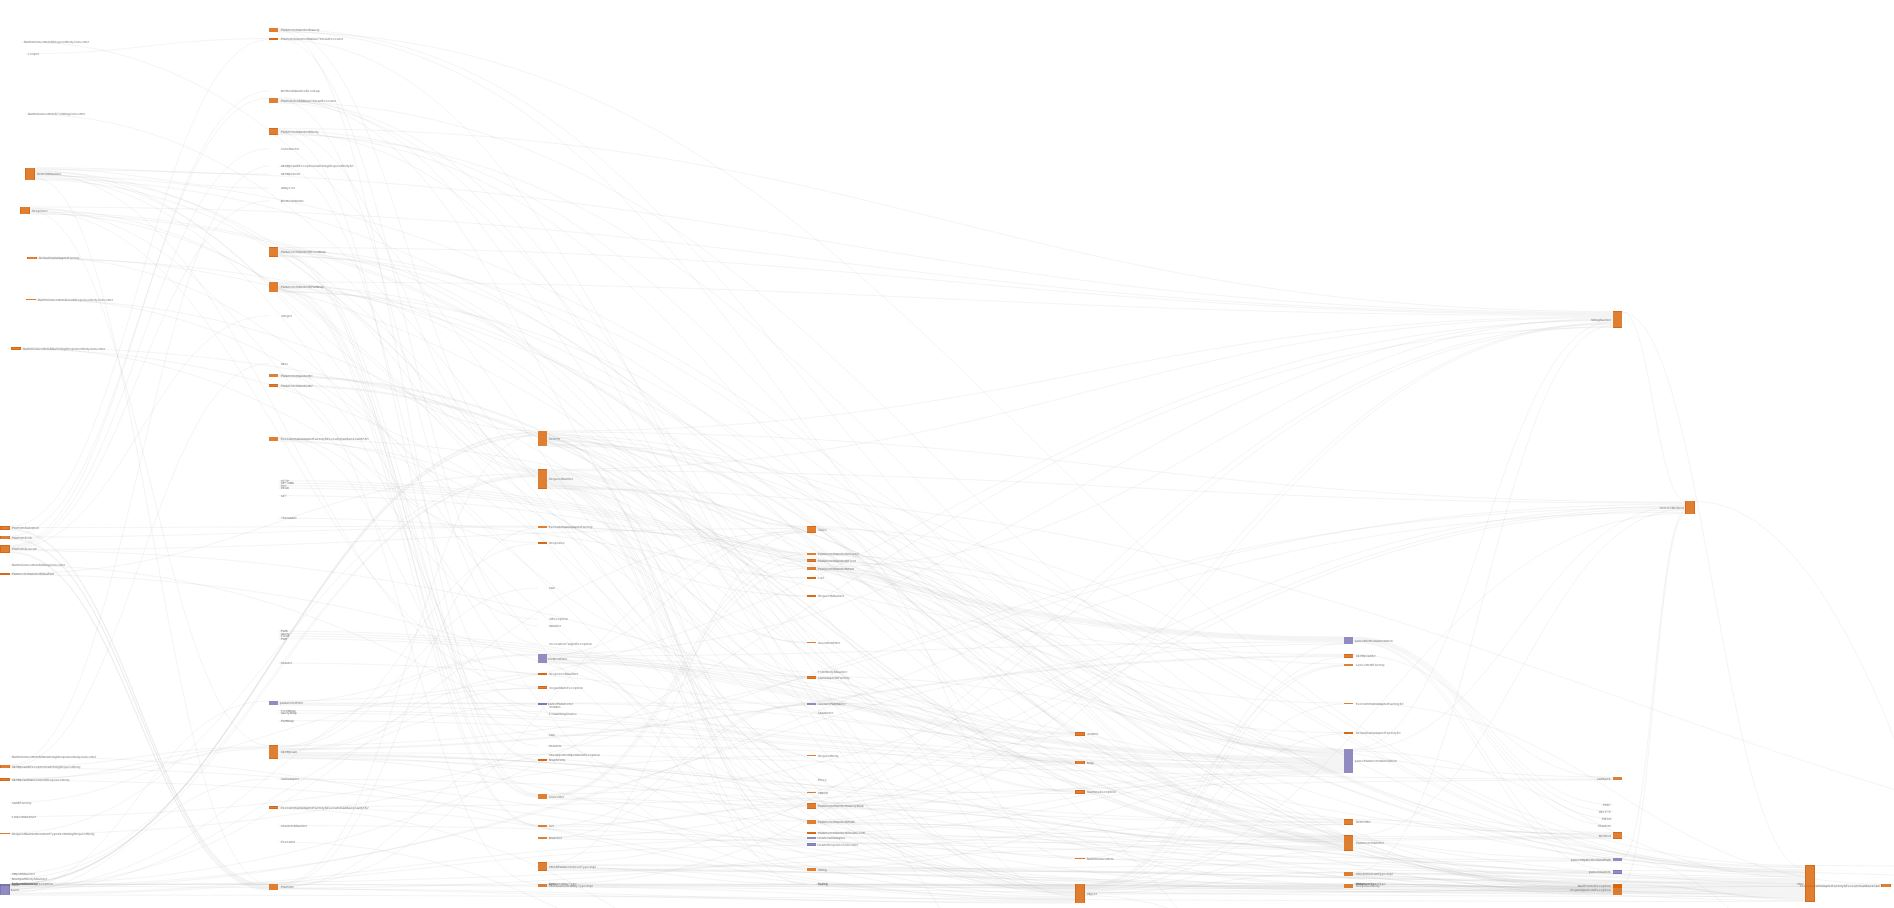
\includegraphics[width=16cm]{graph}
\caption{Noodlr dependency graph for a medium sized project}
\label{fig:graph}
\end{figure*}

\subsection{Threats to Validity}
\label{sec:threats}

\subsubsection{Small Sample Set}

The sample size of pull requests that we used for evaluation is quite small. Although we wrote a script in Ruby\footnote{\url{https://www.ruby-lang.org/en/}} to query Github to extract pull requests using their API, we were limited to manually inspect the pull request data for candidate matches rather than writing a tool to mine this data automatically. This limitation was due to the short amount of time that we had for this project. Future work may include authoring a tool that would effectively mine this data from GitHub and verify the usefulness of our tool in a more efficient manner. Also, even though we gathered data from 4 different projects, we are not claiming that this data is representative of all types of software projects. The 4 projects differ in size and their applicability and also in the number of files available in the pull requests. With a larger sample set of test data that spans several more projects, we would be able to get a better idea of the effectiveness of our tool.

\subsubsection{Developer Behaviors}

All developers are different and with that, most developers have different behaviors. Related to the small sample set limitation described above, we cannot avoid the possibility of using data where the developer behaved in an abnormal manner. For instance, it is completely possible that a developer may have checked-in a large number of files from different part of the project which are not related and the relations between these files would eventually emerge at a later point of time. In this sense, the tool will not be able to predict those files because they are not part of strongly connected components. Our tool does not take this behavior into account as it solely looks at the files belonging to strongly connected components.

\subsubsection{Types of Changes Made}

From exploring hundreds of pull requests, we have noticed that there are several types of software changes that are made where our tool may be more applicable. Generally, for changes that are made where the modifications are in a focused area of a system where components are strongly connected, such as a sub-system component where all parts of the component are related in some way. However, for changes that span a wide area of seemingly unrelated components, or changes such as general comment additions, or spelling corrections, or those things which are unrelated to the Java source files it is difficult for our tool to predict adequately.


\subsubsection{Limitations on D3.js design}

D3 is a open source library which is improved through continuous support of design and data visualization community. For our project also, we had to make some changes in the project to make the Sankey style more interactive with the user. Similarly, there are many other changes that are required in our UI. Most basic issue with current UI of Noodlr is that it cannot support huge projects efficiently. Since the expansion of each node creates many more new child nodes, the screen size becomes an issue after a point. It can be seen in Figure~\ref{fig:graph}, where a medium size project makes it very hard for the user to explore as users will have to scroll and zoom to get a better picture.

\subsubsection{Restriction in the programming language used}

Our tool, in its current state, will work only with projects that use Java as the main programming language. We used tools such as Apache Commons Byte Code Engineering Library (Apache Commons BCEL\texttrademark) for extracting the static call hierarchies. This restricts the scope of our tool. In order to support a new programming language, we will be required to implement language specific tools which can provide us with static call hierarchies. Though, this logic of extracting call hierarchies is a high-level idea that can be used in any programming language, the applicability is severely dependent on the availability of such tools for that programming language. 
